\newpage
\section{Scénario 5 : Scalabilité des réseaux de Petri}
\label{sec:scenario5}

Ce scénario mesure le coût de construction et de traversée de modèles en réseau de Petri de taille croissante via l'API MetaDONE. Deux topologies sont comparées pour isoler l'effet de la connectivité locale des n\oe{}uds, et une optimisation ciblée est proposée, implémentée et évaluée.

% ----------------------------------------------------------------
\subsection{Métamodèle et benchmark}

Le métamodèle \texttt{PetriNet} est créé de façon idempotente via \texttt{PetriNetBootstrap} selon la classe suivante (Listing~\ref{ls-petri}).

\begin{lstlisting}[language=Java, firstnumber=21,
  caption={Bootstrap du métamodèle réseau de Petri},
  label={ls-petri}]
public class PetriNetBootstrap {

    public static MetaModel    mm;
    public static MetaObject   moPlace;
    public static MetaObject   moTransition;
    public static MetaRole     mrArcPT;
    public static MetaRole     mrArcTP;

    public static void setup(Workspace ws) throws BadPreCondition {
        mm           = ws.getMainMetaModel().produceMetaModel("PetriNet");
        moPlace      = mm.produceMetaObject("Place");
        moTransition = mm.produceMetaObject("Transition");
        mrArcPT = mm.produceMetaRole("Arc_PT",
                      MetaRole.Cardinality.MANY_TO_MANY, moPlace, moTransition);
        mrArcTP = mm.produceMetaRole("Arc_TP",
                      MetaRole.Cardinality.MANY_TO_MANY, moTransition, moPlace);
    }
}
\end{lstlisting}

Le métamodèle définit un \texttt{MetaModel} \texttt{mm}, deux \texttt{MetaObject} (\texttt{moPlace} et \texttt{moTransition}) ainsi que deux \texttt{MetaRole} (\texttt{mrArcPT} et \texttt{mrArcTP}) à cardinalité \texttt{MANY\_TO\_MANY}. Cette cardinalité est la plus permissive — aucune contrainte de degré — mais déclenche la précondition DbC \texttt{precondition\_createRole}, qui interdit les paires (domaine, cible) dupliquées pour un même \texttt{MetaRole}.

Deux topologies sont implémentées dans le benchmark.

\paragraph{Topologie 1 — Chaîne cyclique} ($N$ = 100, 500, 1\,000, 5\,000)

Un anneau alternant $N$ places et $N$ transitions, fermé sur lui-même (voir Figure~\ref{fig:sc5-topo1}).

\begin{figure}[h]
\centering
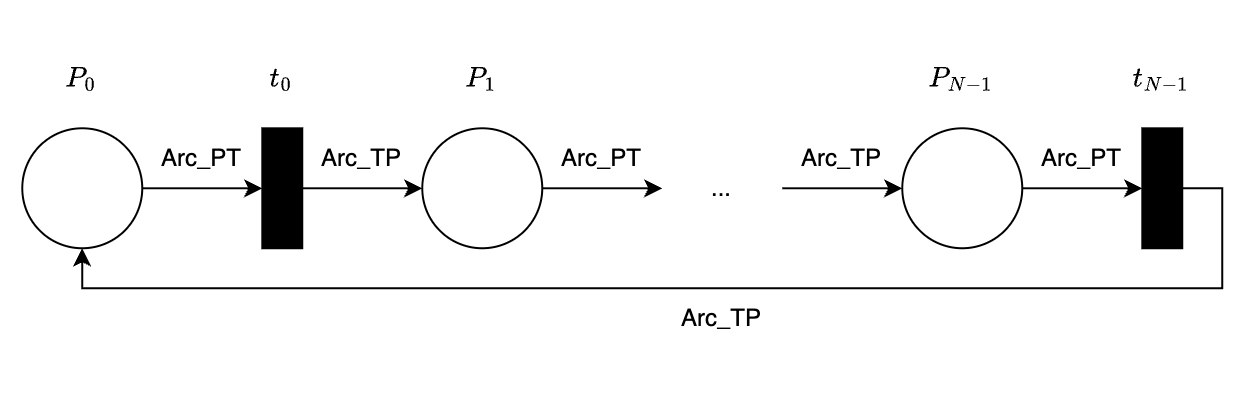
\includegraphics[width=0.6\textwidth]{img/scenario5/topo1.png}
\caption{Topologie 1 : chaîne cyclique}
\label{fig:sc5-topo1}
\end{figure}

Objets : $2N$. Arcs : $2N$ ($N$ \texttt{Arc\_PT} + $N$ \texttt{Arc\_TP}). Degré local de chaque n\oe{}ud : 1 entrant + 1 sortant — constant, indépendant de $N$.

\paragraph{Topologie 2 — Hub} ($N$ = 100, 500, 1\,000)

Une unique \texttt{Transition} centrale connectée à $N$ \texttt{Place}s distinctes (voir Figure~\ref{fig:sc5-topo2}).

\begin{figure}[h]
\centering
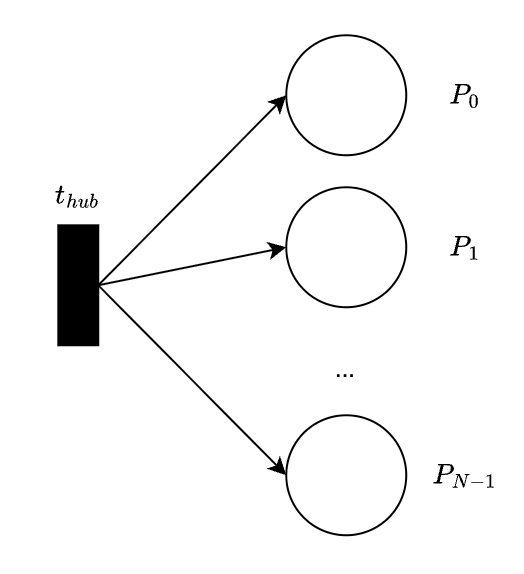
\includegraphics[width=0.25\textwidth]{img/scenario5/topo2.png}
\caption{Topologie 2 : hub central}
\label{fig:sc5-topo2}
\end{figure}

Objets : $N+1$. Arcs : $N$ \texttt{Arc\_TP}. Degré sortant du hub : $N$ — croissant linéairement.

% ----------------------------------------------------------------
\subsection{Résultats de référence (avant optimisation)}

\subsubsection{Création d'objets — chaîne cyclique (2N objets par modèle)}

Le tableau~\ref{tab:sc5-obj-cyclique} présente les médianes obtenues
pour la création de $2N$ objets en topologie cyclique.

\begin{table}[h]
\centering
\caption{Création d'objets --- chaîne cyclique. Médianes calculées sur
10 répétitions (mesures détaillées en annexe~\ref{ann:mesures-s5}).}
\label{tab:sc5-obj-cyclique}
\begin{tabular}{rrrr}
\hline
\textbf{N} & \textbf{Médiane (ms)} & \textbf{µs / objet} & \textbf{CV} \\
\hline
100    & 2,71   & 13,6 & 11,1\,\% \\
500    & 15,68  & 15,7 & 11,8\,\% \\
1\,000 & 26,14  & 13,1 & 16,3\,\% \\
5\,000 & 455,0\textsuperscript{$\dagger$} & 45,5 & 53\,\% \\
\hline
\end{tabular}
\end{table}

\textsuperscript{$\dagger$}\,À $N = 5\,000$, la distribution des dix
mesures est bimodale (5~runs $\approx$~200~ms, 5~runs $\approx$~700~ms),
reflétant l'\emph{entity manager bloat} d'OpenJPA discuté au
chapitre~\ref{chap:discussion}. Une mesure sur workspace fraîchement
initialisé donne $\approx 179$~ms (cohérent avec un coût intrinsèque de
$\sim$\,18~µs/objet).

Pour $N \leq 1\,000$, le coût par objet reste stable autour de
13--16~µs~: \texttt{\_createObject} est bien $O(N)$, conformément au
Scénario~2 (deux INSERTs JPA par objet, sans scan préalable).

\subsubsection{Création d'arcs — chaîne cyclique (2N arcs par modèle)}

Le tableau~\ref{tab:sc5-arc-cyclique} rapporte les temps de création
des arcs en topologie cyclique avant optimisation.

\begin{table}[h]
\centering
\caption{Création d'arcs --- chaîne cyclique, pré-Opt-5A. Médianes sur
10 répétitions (annexe~\ref{ann:mesures-s5}).}
\label{tab:sc5-arc-cyclique}
\begin{tabular}{rrrrc}
\hline
\textbf{N} & \textbf{Arcs} & \textbf{Médiane (ms)} & \textbf{µs / arc} & \textbf{T(N) / N²} \\
\hline
100   & 200     & 3,93       & 19,7  & $3{,}9 \times 10^{-4}$ \\
500   & 1\,000  & 41,57      & 41,6  & $1{,}7 \times 10^{-4}$ \\
1\,000 & 2\,000 & 154,71     & 77,4  & $1{,}5 \times 10^{-4}$ \\
5\,000 & 10\,000 & 4\,481,37 & 448,1 & $1{,}8 \times 10^{-4}$ \\
\hline
\end{tabular}
\end{table}

Le coût par arc double quand $N$ double, et $T(N)/N^2$ converge vers une constante pour $N \geq 500$ : signature d'un comportement $O(N^2)$.

\textit{Observation critique :} la chaîne cyclique, dont chaque n\oe{}ud a un degré local constant de 1, présente le même profil quadratique que le hub à fort degré. Ceci interdit une explication fondée sur la seule connectivité locale.

\subsubsection{Création d'arcs — hub (N arcs Arc\_TP, même n\oe{}ud)}

Le tableau~\ref{tab:sc5-arc-hub} présente les temps mesurés pour la
topologie hub avant optimisation.

\begin{table}[h]
\centering
\caption{Création d'arcs --- hub, pré-Opt-5A. Médianes sur 10
répétitions (annexe~\ref{ann:mesures-s5}).}
\label{tab:sc5-arc-hub}
\begin{tabular}{rrr}
\hline
\textbf{N} & \textbf{Médiane (ms)} & \textbf{µs / arc} \\
\hline
100   & 1,48  & 14,8 \\
500   & 15,72 & 31,4 \\
1\,000 & 63,82 & 63,8 \\
\hline
\end{tabular}
\end{table}

Même croissance $O(N^2)$. À $N = 1\,000$, hub et chaîne cyclique
affichent un coût par arc quasi-identique ($\sim$63--77~µs), révélant
un mécanisme interne commun dominant les deux topologies.

\subsubsection{Traversée — \texttt{getDefinition()} (chaîne cyclique)}

Les modèles cycliques contiennent $4N$ objets : $2N$ places et transitions auxquels s'ajoutent $2N$ \texttt{ConcreteRole}s, les rôles étant eux-mêmes des \texttt{ConcreteObject}s dans la définition du modèle. Le tableau~\ref{tab:sc5-traversal} rapporte les temps mesurés.

\begin{table}[h]
\centering
\caption{Traversée \texttt{getDefinition()} --- chaîne cyclique. Médianes
sur 10 répétitions (annexe~\ref{ann:mesures-s5}).}
\label{tab:sc5-traversal}
\begin{tabular}{rrrrr}
\hline
\textbf{N} & \textbf{Objets trouvés} & \textbf{Médiane (ms)} & \textbf{µs / objet} & \textbf{CV} \\
\hline
100    & 400     &  0,43 & 1,08 & 6,1\,\% \\
500    & 2\,000  &  1,96 & 0,98 & 4,1\,\% \\
1\,000 & 4\,000  &  4,21 & 1,05 & 5,2\,\% \\
5\,000 & 20\,000 & 20,42 & 1,02 & 5,7\,\% \\
\hline
\end{tabular}
\end{table}

La traversée est $O(N)$ à $\sim$1~µs/objet, avec un CV inférieur à 6\,\%
sur toutes les tailles --- parfaitement stable et insensible aux effets
de bloat observés sur la création.

% ----------------------------------------------------------------
\subsection{Analyse de la cause racine}

\subsubsection{Ce que la précondition fait réellement}

La précondition DbC pour \texttt{MANY\_TO\_MANY} dans
\texttt{ConcreteModel\_impl.precondition\_createRole} est la suivante
(Listing~\ref{ls-precond-m2m}).

\begin{lstlisting}[language=Java, firstnumber=386,
  caption={Précondition \texttt{MANY\_TO\_MANY} dans \texttt{precondition\_createRole}},
  label={ls-precond-m2m}]
case MANY_TO_MANY:
    final K_Object robject = range.getTarget();
    for (final K_Property p : domain.getTarget().getDomainOf(theMetaRole)) {
        if (p.getRange().equals(robject)) {
            throw new BadPreCondition(
                "The cardinality of the " + mr.getName()
                + " metarole is violated.");
        }
    }
    break;
\end{lstlisting}

\texttt{getDomainOf(theMetaRole)} itère \texttt{Object\_domainOf} — la liste des rôles \emph{locaux au n\oe{}ud domain} — filtrée par type de \texttt{MetaRole}. Pour la chaîne cyclique, chaque \texttt{Place} possède exactement une entrée \texttt{Arc\_PT} dans \texttt{Object\_domainOf} : le scan est $O(1)$ par appel, $O(N)$ au total. \textbf{La précondition n'est pas la source du $O(N^2)$} pour la topologie cyclique.

\subsubsection{La vraie cause : une asymétrie dans \texttt{\_createRole}}

La lecture en parallèle de \texttt{\_createObject} et \texttt{\_createRole} révèle une différence cruciale.

\texttt{\_createObject} (lignes 57--68 de \texttt{ConcreteModel\_impl}) effectue une \emph{insertion directe} (Listing~\ref{ls-createobject}).

\begin{lstlisting}[language=Java, firstnumber=57,
  caption={Insertion directe dans \texttt{\_createObject}},
  label={ls-createobject}]
private ConcreteObject_impl _createObject(MetaObject_impl metaobject) {
    try {
        final K_Object result = metaobject.getTarget().createObject();
        workspace.getDef_pt().createProperty(result, this.getTarget());
        return FactoryOfProxy.buildConcreteObject(result);
    } ...
}
\end{lstlisting}

\texttt{\_createRole} (lignes 331--345 et son overload ordonné lignes 419--436) passe quant à lui par \texttt{addInDefinition} (Listing~\ref{ls-createrole-avant}).

\begin{lstlisting}[language=Java, firstnumber=331,
  caption={Passage par \texttt{addInDefinition} dans \texttt{\_createRole} (avant optimisation)},
  label={ls-createrole-avant}]
private ConcreteRole_impl _createRole(MetaRole_impl mr,
        ConcreteObject_impl domain, ConcreteObject_impl range) {
    try {
        final K_PropertyType theMetaRole = mr.getMetaroleType();
        final K_Object result_o = mr.getTarget().createObject();
        theMetaRole.createProperty(result_o.getDataObject(),
                domain.getTarget(), range.getTarget());
        final ConcreteRole_impl result =
                FactoryOfProxy.buildConcreteRole(result_o);
        this.addInDefinition(result); // scan O(taille du modele)
        return result;
    } ...
}
\end{lstlisting}

\texttt{\_addInDefinition} appelle \texttt{\_isInDefinition} avant d'insérer (Listing~\ref{ls-addindef}).

\begin{lstlisting}[language=Java, firstnumber=80,
  caption={\texttt{\_addInDefinition} avec vérification préalable},
  label={ls-addindef}]
private ConcreteDef_impl _addInDefinition(ConcreteObject concreteobject) {
    final ConcreteObject_impl coi =
            concreteobject.narrow(ConcreteObject_impl.class);
    if (!_isInDefinition(coi)) {             // cache miss => scan O(N)
        getWorkspace().getDef_pt()
                .createProperty(coi.getTarget(), getTarget());
    }
    cache_isInDefinition.put(coi, true);
    return new ConcreteDef_impl(this, concreteobject);
}
\end{lstlisting}

\texttt{\_isInDefinition}, en cas de cache miss, itère toute la collection \texttt{Object\_rangeOf} du modèle pour vérifier si l'objet est déjà présent. Pour un \texttt{ConcreteRole} fraîchement créé, la réponse est toujours \texttt{false} — il vient d'être instancié et ne peut pas déjà figurer dans la définition. Le scan $O(\text{taille\_du\_modèle})$ est donc \textbf{systématiquement inutile} dans ce contexte.

Quand on crée le $j$-ième arc, le modèle contient déjà $2N + j$ membres ($2N$ objets + $j$ arcs déjà créés). Le scan coûte $O(2N+j)$. La somme sur les $2N$ arcs donne :

$$\sum_{j=0}^{2N-1}(2N+j) \approx 4N^2 + N^2 = 5N^2$$

Ce terme quadratique explique le comportement $O(N^2)$ observé pour les \emph{deux} topologies, indépendamment du degré local. L'asymétrie entre \texttt{\_createObject} (insertion directe) et \texttt{\_createRole} (passage par \texttt{\_addInDefinition}) est la cause racine.

% ----------------------------------------------------------------
\subsection{Optimisation Opt-5A : insertion directe dans \texttt{\_createRole}}

\subsubsection{Description}

Le correctif aligne \texttt{\_createRole} sur le pattern de \texttt{\_createObject} : pour un objet fraîchement créé, le scan \texttt{\_isInDefinition} est supprimé et remplacé par une insertion directe dans la définition du modèle, suivie d'une mise à jour du cache (Listing~\ref{ls-createrole-apres}).

\begin{lstlisting}[language=Java, firstnumber=331,
  caption={\texttt{\_createRole} après Opt-5A},
  label={ls-createrole-apres}]
private ConcreteRole_impl _createRole(MetaRole_impl mr,
        ConcreteObject_impl domain, ConcreteObject_impl range) {
    try {
        final K_PropertyType theMetaRole = mr.getMetaroleType();
        final K_Object result_o = mr.getTarget().createObject();
        theMetaRole.createProperty(result_o.getDataObject(),
                domain.getTarget(), range.getTarget());
        final ConcreteRole_impl result =
                FactoryOfProxy.buildConcreteRole(result_o);
        // result_o est neuf : _isInDefinition est toujours false
        workspace.getDef_pt().createProperty(result_o, this.getTarget());
        cache_isInDefinition.put(result, true);
        return result;
    } ...
}
\end{lstlisting}

Le même correctif est appliqué à l'overload ordonné de \texttt{\_createRole} (ligne 419).

\subsubsection{Propriétés}

\begin{itemize}
  \item \textbf{Correction :} \texttt{result\_o} est créé par \texttt{mr.getTarget().createObject()} — il ne peut pas déjà figurer dans la définition. La suppression du scan est sémantiquement équivalente.
  \item \textbf{DbC :} la précondition \texttt{precondition\_createRole} n'est pas modifiée. Les garanties d'unicité des paires (domaine, cible) restent intégralement assurées.
  \item \textbf{Cache :} la cohérence du \texttt{WeakHashMap} est maintenue via \texttt{cache\_isInDefinition.put(result, true)}, comme dans \texttt{\_addInDefinition}.
  \item \textbf{Portée :} les deux overloads de \texttt{\_createRole} sont corrigés (arcs non ordonnés et ordonnés), soit 4 lignes modifiées au total.
\end{itemize}

% ----------------------------------------------------------------
\subsection{Résultats après optimisation}

\subsubsection{Chaîne cyclique — création d'arcs}

Le tableau~\ref{tab:sc5-arc-cyclique-apres} compare les médianes
avant et après Opt-5A pour la topologie cyclique.

\begin{table}[h]
\centering
\caption{Création d'arcs --- chaîne cyclique, avant et après Opt-5A.
Médianes calculées sur 10 répétitions par campagne
(annexe~\ref{ann:mesures-s5}).}
\label{tab:sc5-arc-cyclique-apres}
\begin{tabular}{rrrrrr}
\hline
\textbf{N} & \textbf{Avant (ms)} & \textbf{Après (ms)} & \textbf{Gain}
           & \textbf{µs/arc avant} & \textbf{µs/arc après} \\
\hline
100    & 3,93       & 3,89      & $\approx 1\times$ & 19,7  & 19,4 \\
500    & 41,57      & 22,02     & $1{,}89\times$    & 41,6  & 22,0 \\
1\,000 & 154,71     & 70,58     & $2{,}19\times$    & 77,4  & 35,3 \\
5\,000 & 4\,481,37  & 1\,021,23 & $4{,}39\times$    & 448,1 & 102,1 \\
\hline
\end{tabular}
\end{table}

Le gain s'accentue avec $N$ --- comportement attendu d'une correction
$O(N^2) \rightarrow O(f(N))$ avec $f(N)$ sous-quadratique.

\textit{Note sur la variabilité à grand $N$ :} la base de données de test
est partagée entre exécutions (singleton \texttt{TestWorkspace}). Au fil
des répétitions, la session OpenJPA accumule des entités persistées par
les exécutions antérieures, ce qui se traduit par un CV plus élevé sur
les phases de création post-Opt-5A ($\sim$\,14\,\% à $N=5\,000$). La
campagne pré-Opt-5A, réalisée immédiatement après revert d'Opt-5A,
montre une stabilité remarquable (CV de 2,8\,\% à $N=5\,000$).

\subsubsection{Complexité résiduelle --- chaîne cyclique}

En comparant les médianes post-Opt-5A à $N = 500$ et $N = 1\,000$~:

$$\frac{T_{\text{arc}}(1\,000)}{T_{\text{arc}}(500)} = \frac{70{,}58}{22{,}02} \approx 3{,}20$$

Pour $O(N)$ pur, on attendrait $2{,}0\times$~; pour $O(N \log N)$,
$\sim 2{,}2\times$~; pour $O(N^2)$, $4{,}0\times$. Le ratio observé
$3{,}20$ se situe entre $O(N \log N)$ et $O(N^2)$~: l'optimisation a
éliminé le coût algorithmique principal mais le plancher mesuré reste
supérieur à $O(N \log N)$ théorique. Cet écart s'explique par la
contribution résiduelle des INSERTs JPA sur l'index B-tree de H2
(chaque insertion dans un index de taille $k$ coûte $O(\log k)$) cumulée
au bruit lié à l'\emph{entity manager bloat} (chapitre~\ref{chap:discussion})~:
le plancher empirique est donc proche de $O(N \log N)$ asymptotique, sans
l'atteindre exactement dans l'environnement de mesure utilisé.

\subsubsection{Hub — création d'arcs}

Le tableau~\ref{tab:sc5-arc-hub-apres} présente le même comparatif
pour la topologie hub.

\begin{table}[h]
\centering
\caption{Création d'arcs --- hub, avant et après Opt-5A. Médianes
calculées sur 10 répétitions par campagne (annexe~\ref{ann:mesures-s5}).}
\label{tab:sc5-arc-hub-apres}
\begin{tabular}{rrrr}
\hline
\textbf{N} & \textbf{Avant (ms)} & \textbf{Après (ms)} & \textbf{Gain} \\
\hline
100    &  1,48 &  1,55 & $\approx 1\times$ \\
500    & 15,72 & 10,99\textsuperscript{$\dagger$} & $1{,}43\times$ \\
1\,000 & 63,82 & 36,16 & $1{,}77\times$    \\
\hline
\end{tabular}
\end{table}

\textsuperscript{$\dagger$}\,À $N=500$, la distribution est bimodale
(six runs $\sim$\,10~ms, quatre runs $\sim$\,34~ms)~; la médiane reflète
la moitié inférieure du cluster.

Le hub bénéficie également du correctif ($\sim$\,1,5--1,7$\times$), mais
reste $O(N^2)$~: la précondition \texttt{MANY\_TO\_MANY} itère désormais
seule \texttt{hub.getDomainOf(Arc\_TP)}, dont la taille croît linéairement
avec le degré. Au $i$-ième arc, le scan coûte $O(i)$~; la somme donne
$O(N^2)$. La mesure confirme cette prédiction~:

$$\frac{N(N-1)}{2}\bigg|_{N=1000} \approx 500\,000 \text{ opérations} \times 72\text{ ns/op} \approx 36{,}0\text{ ms} \quad \text{(mesuré : 36,2~ms)}$$

% ----------------------------------------------------------------
\subsection{Synthèse}

Le tableau~\ref{tab:sc5-synthese} récapitule l'impact d'Opt-5A sur les
deux topologies, les complexités résiduelles et les invariants préservés.

\begin{table}[h]
\centering
\caption{Synthèse Opt-5A. Médianes calculées sur 10 répétitions.}
\label{tab:sc5-synthese}
\begin{tabular}{lll}
\hline
\textbf{Métrique} & \textbf{Avant Opt-5A} & \textbf{Après Opt-5A} \\
\hline
Cyclique --- complexité arcs & $O(N^2)$ & $\sim O(N \log N)$ --- plancher JPA \\
Hub --- complexité arcs      & $O(N^2)$ & $O(N^2)$ --- précondition MANY\_TO\_MANY \\
Cyclique, $N=1\,000$ arcs    & 155 ms     & \textbf{71 ms} ($2{,}19\times$) \\
Cyclique, $N=5\,000$ arcs    & 4\,481 ms  & \textbf{1\,021 ms} ($4{,}39\times$) \\
Traversée                    & $O(N)$, $\sim$1~µs/objet & inchangée \\
DbC                          & intact     & intact \\
Lignes modifiées             & ---        & 4 lignes, 2 méthodes \\
\hline
\end{tabular}
\end{table}

% ----------------------------------------------------------------
\subsection{Bottleneck résiduel — hub (non implémenté)}

Pour ramener la topologie hub à $O(N \log N)$, il faudrait un second correctif dans \texttt{pre\-con\-di\-tion\_crea\-te\-Role} : remplacer l'itération de \texttt{getDomainOf(theMetaRole)} par un lookup $O(1)$ dans un index maintenu dans \texttt{ConcreteModel\_impl} (Listing~\ref{ls-roleindex}).

\begin{lstlisting}[language=Java,
  caption={Index proposé pour \texttt{precondition\_createRole} MANY\_TO\_MANY},
  label={ls-roleindex}]
// Dans ConcreteModel_impl
private final Map<K_PropertyType,
                  Map<K_Object, Set<K_Object>>> roleIndex = new HashMap<>();

// Dans precondition_createRole, cas MANY_TO_MANY :
Set<K_Object> ranges = roleIndex
    .getOrDefault(theMetaRole, Collections.emptyMap())
    .getOrDefault(domain.getTarget(), Collections.emptySet());
if (ranges.contains(range.getTarget())) {
    throw new BadPreCondition("...");
}

// Dans _createRole, apres l'insertion :
roleIndex.computeIfAbsent(theMetaRole, k -> new HashMap<>())
         .computeIfAbsent(domain.getTarget(), k -> new HashSet<>())
         .add(range.getTarget());
\end{lstlisting}

Cette approche nécessite une initialisation \emph{lazy} de l'index lors de la première vérification pour les modèles chargés depuis la base, ainsi qu'une invalidation à la suppression de rôles. L'implémentation est plus invasive et sort du périmètre du présent scénario.

% ----------------------------------------------------------------
\subsection{Conclusion}

Le Scénario~5 révèle et corrige une inefficacité cachée dans la création de rôles de MetaDONE. La cause racine est une asymétrie de conception entre \texttt{\_createObject} (insertion directe en $O(1)$) et \texttt{\_createRole} (passage par \texttt{\_addInDefinition} $\rightarrow$ scan $O(\text{taille\_du\_modèle})$), rendant toute création de rôle $O(N^2)$ quelle que soit la topologie du modèle.

L'optimisation Opt-5A, réalisée dans deux méthodes de \texttt{ConcreteModel\_impl}, aligne \texttt{\_createRole} sur \texttt{\_createObject} en supprimant un scan systématiquement inutile pour des objets fraîchement créés. Elle réduit la complexité de la création d'arcs de $O(N^2)$ à un plancher proche de $O(N \log N)$ pour les topologies à degré borné, avec un gain empirique médian de $2{,}19\times$ à $N = 1\,000$ et $4{,}39\times$ à $N = 5\,000$ (mesuré sur 10 répétitions par campagne). La sémantique DbC est intégralement préservée.

Pour les tailles de modèles typiques de MetaDONE ($N < 200$), les performances étaient déjà acceptables. Le bénéfice est significatif dès $N \geq 500$ et devient critique à $N = 5\,000$, où la création de $10\,000$ arcs en chaîne cyclique passe de $4\,481$~ms à $1\,021$~ms (cf.~tableau~\ref{tab:sc5-arc-cyclique-apres}), rendant la construction de grands modèles de vérification formelle praticable dans un contexte interactif.
